\section{IR of Industrial Compilers}
\frame{
\frametitle{IR of Industrial Compilers :: LLVM Bitcode \\
How to generate IR for function calls?
}
\begin{columns}
\begin{column}{0.60\textwidth}
\begin{center}
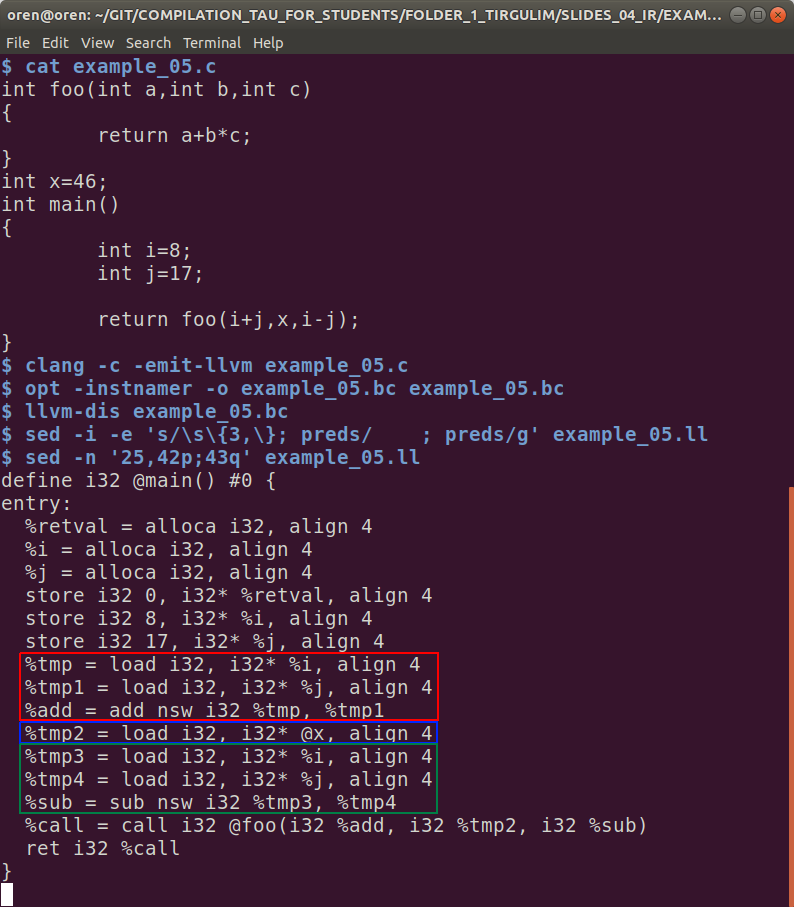
\includegraphics[width=0.95\textwidth]{example_05.png}
\end{center}
\end{column}
\begin{column}{0.6\textwidth}
\begin{itemize}
\item
3 parameters are sent for foo:
\begin{itemize}
\item add = i $+$ j ({\color{red} red})
\item tmp2 = x      ({\color{blue} blue})
\item sub = i $-$ j ({\color{green} green})
\end{itemize}
\item
does evaluation order matter?
\item
how should we handle \\
the return value?
\item
which calling convention \\
is implied here?
\item
which calling convention \\
should we adopt          \\
in \textit{our} project?
\end{itemize}
\end{column}
\end{columns}
}